\documentclass[10pt,a4paper]{article}
\usepackage[margin=21mm,headheight=15pt]{geometry}
\usepackage[T1]{fontenc}
\usepackage{lmodern,amsmath,amssymb,tikz,graphicx,hyperref,fancyhdr,enumitem}
\usetikzlibrary{arrows.meta,positioning,calc,decorations.pathmorphing}
\definecolor{ink}{RGB}{20,53,78}
\hypersetup{colorlinks=true,urlcolor=ink,linkcolor=ink}
\setlength{\parindent}{0pt}\setlength{\parskip}{5pt}
\emergencystretch=3em
\pagestyle{fancy}\fancyhf{}\fancyfoot[C]{\thepage}
\renewcommand{\headrulewidth}{.3pt}
\newcommand{\task}[2]{\par\medskip{\color{ink}\Large\bfseries #1. #2}\par\smallskip}
\newcommand{\answer}{\par\smallskip\textbf{Worked reasoning.} }
\setlist[enumerate]{label=\textbf{(\alph*)},leftmargin=7mm,itemsep=7pt}
\begin{document}
\fancyhead[L]{\small Control of Dynamical Systems}
\fancyhead[R]{\small Laboratory 09}
{\color{ink}\LARGE\bfseries Laboratory 09}\par
{\large PID regulation when the actuator saturates}\par
\textbf{Exercise sheet -- five integrated problems}\par
{\small\textbf{Evidence boundary.} Original hypothetical scenarios. Derive, calculate and justify decisions; every numerical record is synthetic. Figures are conceptual and not to scale.}
\smallskip\textbf{Shared nominal data.} Nominal plant: $\ddot y+2\dot y+y=u$. The physical realization has $m=1$ kg, $b=2$ N s/m and $k=1$ N/m. Ideal PID pole targets are $-2,-3,-4$; constrained cases impose $|u|\le2$.
\task{1}{Pole placement for a force-limited positioning stage}
The physical illustration gives one realization of $\ddot y+2\dot y+y=u$: a 1 kg carriage, a 2 N s/m damper and a 1 N/m spring, driven by an ideal force actuator. Position is in m and force in N.
\begin{center}\resizebox{\ifdim\width>.98\linewidth.98\linewidth\else\width\fi}{!}{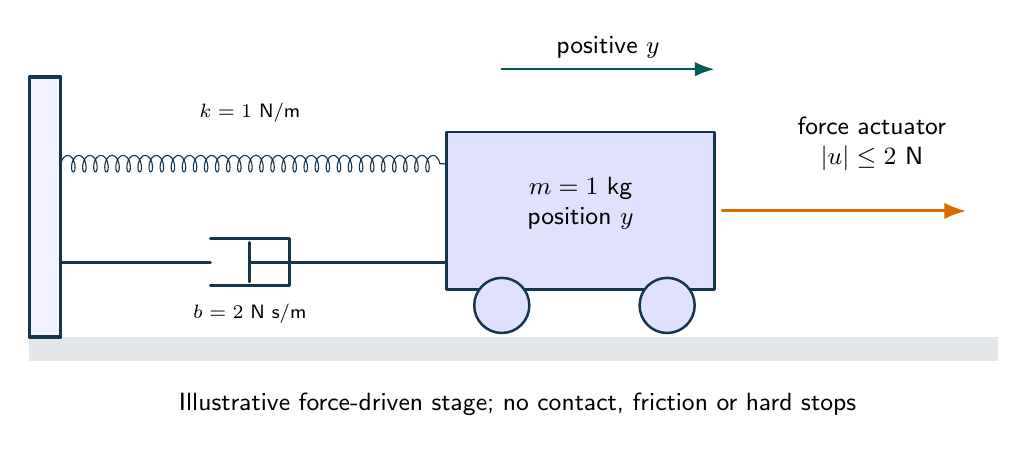
\begin{tikzpicture}[
font=\sffamily\small,>=Latex,line cap=round,line join=round,
wall/.style={draw=ink,line width=1.2pt,fill=blue!5},
water/.style={fill=cyan!25,draw=none},
metal/.style={draw=ink,fill=blue!12,line width=.9pt},
flow/.style={->,draw=blue!65!black,line width=1.2pt},
heat/.style={->,draw=orange!85!black,line width=1.1pt},
measure/.style={->,draw=teal!70!black,line width=.9pt},
dim/.style={<->,draw=ink!65,line width=.6pt},
spring/.style={draw=ink,decorate,decoration={coil,aspect=.5,segment length=4pt,amplitude=3pt}},
wire/.style={draw=ink,line width=1pt},
lab/.style={align=center,font=\sffamily\small},
smalllab/.style={align=center,font=\sffamily\scriptsize}]

\fill[ink!12](.7,.4)rectangle(13,.7);
\draw[wall](.7,.7)rectangle(1.1,4);
\draw[metal](6,1.3)rectangle(9.4,3.3);
\node[lab]at(7.7,2.4){$m=1$ kg\\position $y$};
\draw[spring](1.1,2.9)--(6,2.9);
\node[smalllab]at(3.5,3.55){$k=1$ N/m};
\draw[wire](1.1,1.65)--(3,1.65)(3,1.35)--(4,1.35)--(4,1.95)--(3,1.95);
\draw[wire](6,1.65)--(3.5,1.65)(3.5,1.4)--(3.5,1.9);
\node[smalllab]at(3.5,1){$b=2$ N s/m};
\draw[metal](6.7,1.1)circle(.35)(8.8,1.1)circle(.35);
\draw[heat](9.5,2.3)--(12.6,2.3);
\node[lab]at(11.4,3.15){force actuator\\$|u|\leq2$ N};
\draw[measure](6.7,4.1)--(9.4,4.1)node[midway,above]{positive $y$};
\node[lab]at(6.9,-.15){Illustrative force-driven stage; no contact, friction or hard stops};
\end{tikzpicture}
}\par{\small A mass, spring, damper and bounded force actuator physically realize the normalized second-order plant. Force saturation is included; contact, dry friction and travel stops are not.}\end{center}
\begin{enumerate}
\item For $G=1/(s^2+2s+1)$, use ideal PID $C=k_p+k_i/s+k_ds$. Match the closed-loop denominator to $(s+2)(s+3)(s+4)$ and find all three gains.
\item Compare $u=k_pe+k_i\int e\,dt+k_d\dot e$ with $u=k_pe+k_i\int e\,dt-k_d\dot y$, where $e=r-y$. Derive both reference numerators for the preceding plant and explain derivative kick.
\item For a 3 m reference step, determine the impulsive contribution requested by ideal derivative-on-error action with the designed $k_d$. Explain why matching the nominal poles does not make that command physically realizable.
\end{enumerate}
\vfill{\small\textbf{Submission.} Show the model, intermediate reasoning, units and a conclusion addressing the stated requirements.}

\newpage
\task{2}{Implementing a filtered controller as a state model}
Replace the ideal derivative by a first-order filter and retain the resulting additional dynamics. Compare a transfer-function calculation with a state-equation calculation.
\begin{enumerate}
\item Use derivative-on-measurement $D_f=7s/(0.03s+1)$. Derive a first-order filter-state implementation and its high-frequency gain. Give the units of the filter time constant.
\item With gains 25, 24 and 7 and filter constant 0.03, derive the unsaturated characteristic polynomial. Verify strict stability using the quartic Routh inequalities.
\item Use states $[y,v,z,I]^T$, where $v=\dot y$ and $\tau_f\dot z=y-z$. Derive the unsaturated zero-reference state matrix and explain how its eigenvalues check the filtered characteristic polynomial.
\end{enumerate}
\vfill{\small\textbf{Submission.} Show the model, intermediate reasoning, units and a conclusion addressing the stated requirements.}

\newpage
\task{3}{An unreachable reference with a bounded integral state}
The requested position exceeds the equilibrium capability of the force actuator. Analyze both ordinary integration and back-calculation without confusing bounded controller state with successful tracking.
\begin{center}\resizebox{\ifdim\width>.98\linewidth.98\linewidth\else\width\fi}{!}{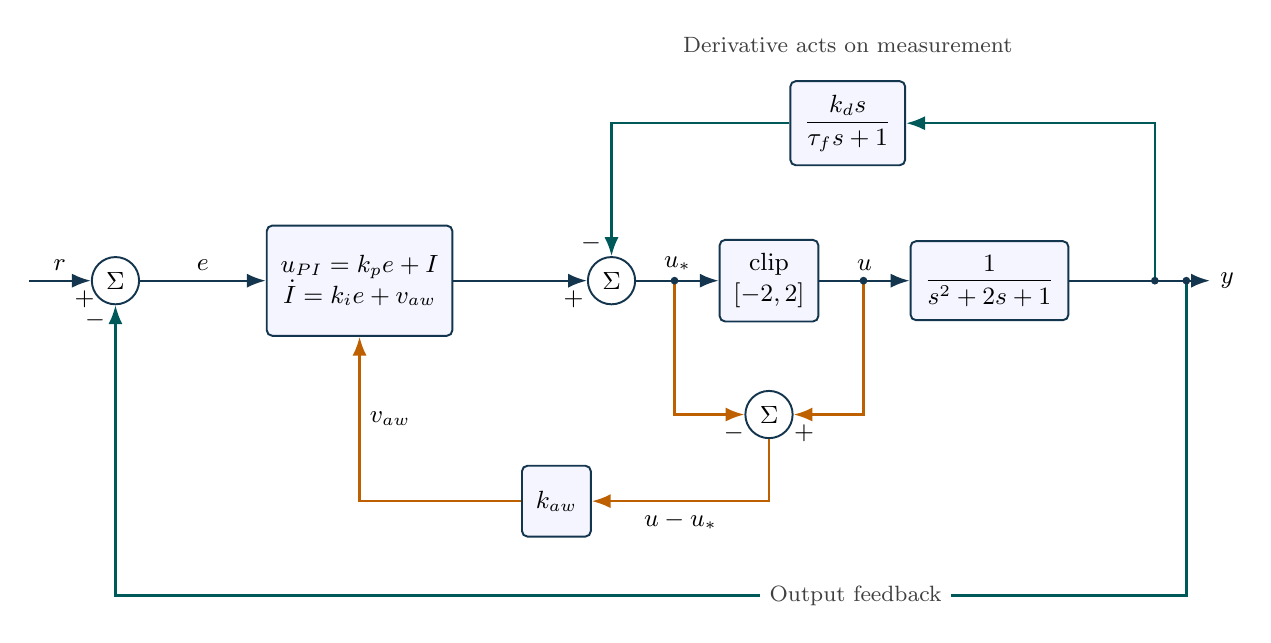
\begin{tikzpicture}[x=1cm,y=1cm,>=Latex,font=\small,
block/.style={draw=ink,fill=blue!4,rounded corners=2pt,minimum height=9mm,align=center,line width=.7pt,inner sep=5pt},
sum/.style={circle,draw=ink,fill=white,minimum size=6mm,inner sep=0pt,line width=.7pt},
sig/.style={->,draw=ink,line width=.85pt},
fb/.style={->,draw=teal!70!black,line width=.85pt},
dist/.style={->,draw=orange!75!black,line width=.85pt},
tap/.style={circle,fill=ink,inner sep=1.4pt},
note/.style={font=\footnotesize,align=center,text=black!75}]

\node[sum](e)at(.9,0){$\Sigma$};
\node[block,minimum height=14mm](pi)at(4,0){$u_{PI}=k_pe+I$\\$\dot I=k_ie+v_{aw}$};
\node[sum](tot)at(7.2,0){$\Sigma$};
\node[block](sat)at(9.2,0){$\operatorname{clip}$\\$[-2,2]$};
\node[block](plant)at(12,0){$\dfrac{1}{s^2+2s+1}$};
\draw[sig](-.2,0)--node[above]{$r$}node[pos=.9,below]{$+$}(e);
\draw[sig](e)--node[above]{$e$}(pi);
\draw[sig](pi)--node[pos=.9,below]{$+$}(tot);
\draw[sig](tot)--node[above]{$u_*$}(sat);
\draw[sig](sat)--node[above]{$u$}(plant);
\draw[sig](plant)--(14.8,0)node[right]{$y$};
\node[block](df)at(10.2,2){$\dfrac{k_ds}{\tau_fs+1}$};
\draw[fb](14.1,0)--(14.1,2)--(df);
\draw[fb](df)--(7.2,2)--node[pos=.9,left]{$-$}(tot);
\fill[ink](14.1,0)circle(1.4pt);
\node[note]at(10.2,3){Derivative acts on measurement};
\node[sum](aw)at(9.2,-1.7){$\Sigma$};
\draw[dist](10.4,0)--(10.4,-1.7)--node[pos=.85,below]{$+$}(aw);
\draw[dist](8,0)--(8,-1.7)--node[pos=.85,below]{$-$}(aw);
\fill[ink](10.4,0)circle(1.4pt);\fill[ink](8,0)circle(1.4pt);
\node[block](kaw)at(6.5,-2.8){$k_{aw}$};
\draw[dist](aw)--(9.2,-2.8)--node[below]{$u-u_*$}(kaw);
\draw[dist](kaw)--(4,-2.8)--node[right]{$v_{aw}$}(pi.south);
\draw[fb](14.5,0)--(14.5,-4)--(.9,-4)--node[pos=.95,left]{$-$}(e);
\fill[ink](14.5,0)circle(1.4pt);
\node[note,fill=white]at(10.3,-4){Output feedback};

\end{tikzpicture}
}\par{\small Filtered derivative acts on measurement. Back-calculation sends the actual-minus-requested actuator effort into the integral-state equation.}\end{center}
\begin{enumerate}
\item The plant satisfies $\ddot y+2\dot y+y=u$ and the actuator is limited to $[-2,2]$. Is a constant reference of 3 feasible? What is the largest positive equilibrium output, and what happens to an ordinary integral state if the tracking error stays at one?
\item Use $\dot I=24e+k_{aw}(u-u_*)$ with $k_{aw}=8$. At an instant when $e=1$, requested effort $u_*=5$ and saturated effort $u=2$, evaluate $\dot I$. Find the request excess that balances integration for a constant positive error e.
\item Find a saturated steady state for $r=3$, $u_{\max}=2$ and $k_{aw}=8$, including $y,v,z,I,u_*$, for the filtered derivative-on-measurement implementation. State the remaining tracking error.
\end{enumerate}
\vfill{\small\textbf{Submission.} Show the model, intermediate reasoning, units and a conclusion addressing the stated requirements.}

\newpage
\task{4}{Anti-windup speed and numerical step-size limits}
During a fixed saturation interval, the anti-windup correction can be faster than the plant. Examine that local time scale before choosing a numerical integrator.
\begin{enumerate}
\item Assume, only for this local calculation, that $e=0.4$ and $u-u_*=-0.5$ remain constant for 2 s. Find the integral-state increment with and without back-calculation gain 8. Explain the scope of this calculation.
\item Hold y, r and the filtered derivative contribution fixed while the actuator remains at a fixed saturation limit. Derive the homogeneous dynamics of a perturbation in integral state I. Compare its time constant for gains 8 and 40.
\item Apply explicit Euler to the homogeneous local integral-state perturbation. Derive the strict step-size condition for its decay and evaluate it for gains 8 and 40. Explain why satisfying this condition alone is insufficient for the full simulation.
\end{enumerate}
\vfill{\small\textbf{Submission.} Show the model, intermediate reasoning, units and a conclusion addressing the stated requirements.}

\newpage
\task{5}{A reproducible recovery comparison with an explicit evidence limit}
The reference becomes feasible after an initial saturated interval. Compare recovery using both tracking and actuator records, keeping all data explicitly synthetic.
\begin{enumerate}
\item A synthetic experiment commands 3 until 6 s, then 0.2 until 12 s. Define recovery IAE on the second interval. Given values 9.756216 without back-calculation and 1.841207 with it, calculate the percentage reduction and discuss what the metric omits.
\item Specify a numerical protocol for comparing the two anti-windup settings fairly. Include the reference discontinuity, time resolution, metrics and the evidence label. Explain why plotting only the requested effort is insufficient.
\item Suppose a design objective is $J={\rm IAE}+\lambda\int_6^{12}\dot u(t)^2\,dt$ with $\lambda>0$. Can the supplied two IAE values alone rank the controllers under this objective? Specify the additional records and numerical care required.
\end{enumerate}
\vfill{\small\textbf{Submission.} Show the model, intermediate reasoning, units and a conclusion addressing the stated requirements.}

\end{document}
